\documentclass[10pt,letterpaper]{article}

% --- Paquetes de configuración y tipografía ---
\usepackage[utf8]{inputenc}
\usepackage[T1]{fontenc}
\usepackage{lmodern}
\usepackage[letterpaper,top=2.0cm,bottom=2.0cm,left=2.0cm,right=2.0cm,headheight=20pt,headsep=12pt]{geometry}
% babel omitido

% --- Matemáticas, símbolos y gráficos ---
\usepackage{amsmath,amssymb}
\usepackage{booktabs}
\usepackage{tabularx}
\usepackage{longtable}
\usepackage{pdflscape}
\usepackage{array}
\usepackage{graphicx}
\usepackage{xcolor}
\usepackage{colortbl}
\usepackage{fancyhdr}
\usepackage{tcolorbox}
\tcbuselibrary{skins,breakable}
\usepackage{hyperref}
\usepackage{titlesec}
\usepackage{enumitem}
\usepackage{lastpage}
\usepackage{caption}
\captionsetup[table]{name=Cuadro,labelfont=bf,textfont=bf}
\captionsetup[figure]{name=Figura,labelfont=bf,textfont=bf}
\usepackage{float}
\usepackage{tikz}
\usetikzlibrary{arrows.meta,shapes.geometric,positioning,calc}

% --- Colores Corporativos Solvanta Engineering Solutions ---
\definecolor{solvantablue}{RGB}{14, 54, 95}     % #0e365f - Azul Institucional
\definecolor{solvantateal}{RGB}{28, 110, 128}   % #1c6e80 - Teal Secundario
\definecolor{solvantagreen}{RGB}{46, 125, 50}   % #2e7d32 - Verde Sostenible
\definecolor{lightbg}{RGB}{246, 249, 252}       % #f6f9fc - Fondo Suave
\definecolor{cardborder}{RGB}{205, 220, 233}    % Borde cajas
\definecolor{rowgray}{RGB}{248, 250, 252}       % Filas alternas
\definecolor{alertred}{RGB}{185, 28, 28}        % Alarmas críticas

% --- Configuración de Hipervínculos ---
\hypersetup{
    colorlinks=true,
    linkcolor=solvantablue,
    citecolor=solvantateal,
    urlcolor=solvantablue,
    pdfauthor={Solvanta Engineering Solutions S.A. de C.V.},
    pdftitle={FC-01 Filosofia de Control del Proceso - Planta de e-Metanol}
}

% --- Encabezados y Pies de Página ---
\pagestyle{fancy}
\fancyhf{}
\renewcommand{\headrulewidth}{0.5pt}
\renewcommand{\footrulewidth}{0.5pt}
\renewcommand{\headrule}{\hbox to\headwidth{\color{solvantablue}\leaders\hrule height \headrulewidth\hfill}}
\renewcommand{\footrule}{\hbox to\headwidth{\color{solvantablue}\leaders\hrule height \footrulewidth\hfill}}

\fancyhead[L]{\small\bfseries\color{solvantablue} Solvanta Engineering Solutions \quad\textbar\quad DPyPQ}
\fancyhead[R]{\small\bfseries\color{solvantablue} FC-01: Filosofía de Control del Proceso}
\fancyfoot[L]{\footnotesize\color{gray} Planta de e-Metanol ($30\,000\text{ t/año}$) \textbar\ RFP-CCM-EM-001}
\fancyfoot[C]{\footnotesize\color{solvantablue}\textbf{Página \thepage\ de \pageref{LastPage}}}
\fancyfoot[R]{\footnotesize\color{gray} BUAP \textbar\ Fac. de Ing. Química}

% --- Formato de Títulos ---
\titleformat{\section}{\large\bfseries\color{solvantablue}}{\thesection.}{0.5em}{}
\titleformat{\subsection}{\normalsize\bfseries\color{solvantateal}}{\thesubsection.}{0.5em}{}
\titleformat{\subsubsection}{\small\bfseries\color{solvantablue}}{\thesubsubsection.}{0.5em}{}
\titlespacing*{\section}{0pt}{8pt}{4pt}
\titlespacing*{\subsection}{0pt}{6pt}{3pt}
\titlespacing*{\subsubsection}{0pt}{4pt}{2pt}

\setlist{nosep,leftmargin=1.3em}
\setlength{\parindent}{0pt}
\setlength{\parskip}{4pt}

% Columnas personalizadas
\newcolumntype{L}[1]{>{\raggedright\arraybackslash}p{#1}}
\newcolumntype{C}[1]{>{\centering\arraybackslash}p{#1}}
\newcolumntype{R}[1]{>{\raggedleft\arraybackslash}p{#1}}

\begin{document}

% ==============================================================================
% PORTADA OFICIAL DE LA FIRMA DE INGENIERÍA
% ==============================================================================
\begin{titlepage}
\begin{center}
    \vspace*{-0.5cm}
    {\large \textbf{BENEMÉRITA UNIVERSIDAD AUTÓNOMA DE PUEBLA}}\\[0.2cm]
    {\large \textbf{FACULTAD DE INGENIERÍA QUÍMICA}}\\[0.3cm]
    {\normalsize \textbf{Colegio de Ingeniería Química \quad\textbar\quad Otoño 2026}}\\[0.8cm]

    \begin{tcolorbox}[colback=solvantablue,colframe=solvantablue,arc=2mm,coltext=white,boxrule=0pt,center,width=0.95\textwidth]
        \begin{center}
            \vspace{0.2cm}
            {\LARGE \textbf{FC-01}}\\[0.3cm]
            {\Large \textbf{FILOSOFÍA DE CONTROL DEL PROCESO}}\\[0.2cm]
            \vspace{0.1cm}
            {\normalsize \textbf{Asignatura:} Diseño de Procesos y Productos Químicos}\\[0.1cm]
            {\footnotesize Documento Técnico de Ingeniería Básica e Instrumentación de Proceso}
            \vspace{0.2cm}
        \end{center}
    \end{tcolorbox}

    \vspace{0.6cm}
    \begin{minipage}{0.9\textwidth}
        \centering
        \textbf{Firma de Ingeniería:}\\[0.1cm]
        {\large \textbf{\color{solvantablue} Solvanta Engineering Solutions S.A. de C.V.}}\\[0.15cm]
        \textit{"Soluciones que transforman la industria"}\\[0.4cm]
        
        \textbf{Nombre del Proyecto:}\\[0.1cm]
        {\large \textbf{Planta de Producción de e-Metanol Grado Químico AA ($30\,000\text{ t/año}$)}}\\[0.1cm]
        {\normalsize Síntesis Catalítica a partir de $\text{CO}_2$ Capturado e Hidrógeno Electrolítico SOEC}\\[0.15cm]
        \textbf{Referencia de Licitación:} RFP-CCM-EM-001\\[0.4cm]
        
        \textbf{Proceso:}\\[0.1cm]
        {\normalsize Producción de metanol}\\[0.6cm]
        
        \textbf{Integrantes del Equipo de Ingeniería:}\\[0.2cm]
        \begin{tabular}{ll}
            \toprule
            \textbf{Nombre Completo} & \textbf{Especialidad / Rol en el Proyecto} \\
            \midrule
            \textbf{Karol Paola Camacho López} & Dirección de Proyecto / Python \& Optimización \\
            \textbf{Gildardo Ocaña Barrales} & Ingeniería de Procesos / AutoCAD Plant 3D \& DTI \\
            \textbf{Paulina Mota Macip} & Simulación DWSIM / Instrumentación \& Control \\
            \textbf{Grecia Figueroa Rincón} & Evaluación Económica / BioSTEAM \& HSE/Seguridad \\
            \bottomrule
        \end{tabular}\\[0.6cm]
        
        \textbf{Profesor Titular:}\\[0.1cm]
        {\normalsize Cátedra de Diseño de Procesos y Productos Químicos}\\[0.3cm]
        
        \textbf{Fecha de Emisión Oficial:}\\[0.1cm]
        {\normalsize 5 de octubre de 2026 \quad\textbar\quad Puebla, Pue., México}
    \end{minipage}

    \vfill
    \begin{tcolorbox}[colback=lightbg,colframe=solvantateal,arc=1.5mm,width=0.95\textwidth,boxrule=0.8pt]
        \footnotesize \textbf{Nota de Confidencialidad y Control Documental:} El presente documento técnico ha sido elaborado por Solvanta Engineering Solutions con base en el modelo termodinámico riguroso convergido en DWSIM v1, los balances de materia y energía del proyecto RFP-CCM-EM-001 y las capturas de instrumentación de campo verificadas.
    \end{tcolorbox}
\end{center}
\end{titlepage}

% ==============================================================================
% SECCIÓN 1: INTRODUCCIÓN Y CONCEPTOS BÁSICOS
% ==============================================================================
\section{Introducción}
Durante el diseño de un proceso químico industrial no es suficiente definir los balances de materia y energía estacionarios, las dimensiones de los equipos o la disposición de las corrientes. La operación real de una planta química está sujeta a perturbaciones intrínsecas: fluctuaciones en las condiciones ambientales, variaciones de pureza o presión en las materias primas, ensuciamiento paulatino de las superficies de transferencia de calor y desviaciones dinámicas de carga. 

Para asegurar que la planta opere de forma continua, segura, económica y dentro de los estrictos límites de calidad del producto final (e-metanol grado AA, pureza $>99.85\,\%\text{ p/p}$, según norma ASTM D1152), es indispensable formular la \textbf{filosofía de control del proceso}. Este documento establece la lógica operacional, la selección de variables a gobernar, la jerarquía de los lazos regulatorios y las acciones protectoras de salvaguarda.

\section{¿Qué es una Filosofía de Control?}
La filosofía de control es el documento de ingeniería básica que define formalmente cómo se pretende operar, regular y proteger un proceso químico para mantenerlo estable y dentro de su envolvente de diseño admisible. En particular, este documento determina:
\begin{itemize}
    \item \textbf{Variables a medir:} Identificación de sensores primarios de temperatura ($T$), presión ($P$), caudal ($F$), nivel de líquido ($L$), composición ($x, y$) y margen de inestabilidad mecánica.
    \item \textbf{Variables a controlar:} Parámetros críticos del proceso cuyo valor debe permanecer fijo en una consigna (*setpoint*, SP) o acotado en una banda de tolerancia operativa.
    \item \textbf{Variables a manipular:} Caudales de fluidos, potencias eléctricas o aperturas de válvulas de control que el sistema ajusta dinámicamente para contrarrestar las desviaciones.
    \item \textbf{Respuesta del sistema:} Sentido de la acción correctiva ante perturbaciones (acción directa o inversa en controladores y acción de falla de válvulas).
    \item \textbf{Estrategia de alarmas e interlocks:} Criterios de alerta temprana para el operador (alarmas bajas y altas) y disparos de seguridad de actuación automática independientes para evitar condiciones catastróficas.
\end{itemize}

\section{Relación entre Filosofía de Control y DTI (P\&ID)}
Existe una relación secuencial directa e indisoluble entre la filosofía de control y el Diagrama de Tuberías e Instrumentación (DTI):
\begin{center}
\begin{tcolorbox}[colback=lightbg,colframe=solvantablue,arc=1.5mm,width=0.85\textwidth,boxrule=0.8pt]
    \centering
    \textbf{Secuencia Metodológica de Ingeniería:}\\[0.15cm]
    $\text{FC-01 (Filosofía de Control)} \longrightarrow \text{DTI v0.1} \longrightarrow \text{HAZOP} \longrightarrow \text{Matriz Causa-Efecto} \longrightarrow \text{DTI v1.0}$
\end{tcolorbox}
\end{center}
Primero se decide conceptualmente la estrategia de gobernanza del proceso (\textit{¿Cómo queremos controlar la planta?}) y posteriormente se representa físicamente en el DTI (\textit{¿Cómo implementaremos los instrumentos, señales y válvulas en tuberías y recipientes?}). En el DTI cada estrategia se plasma mediante símbolos normalizados ANSI/ISA-5.1:
\begin{equation*}
    \text{Sensor/Transmisor (TT/PT/LT/FT)} \longrightarrow \text{Controlador (TIC/PIC/LIC/FIC)} \longrightarrow \text{Elemento Final (TCV/PCV/LCV/FCV)}
\end{equation*}

\section{Objetivo de la Actividad}
Desarrollar la \textbf{filosofía de control preliminar del proceso de síntesis de e-metanol ($30\,000\text{ t/año}$)} diseñado por Solvanta Engineering Solutions, identificando las variables críticas de operación, las estrategias de control multivariable y en cascada, las principales perturbaciones, las alarmas preventivas y las acciones de protección por interlock. La información generada constituye la base técnica vinculante para la actualización del DTI oficial del proyecto, el futuro estudio HAZOP y la formulación de la matriz causa-efecto.

\section{Información Técnica Utilizada}
El desarrollo del presente documento se sustenta rigurosamente en la evidencia técnica generada y verificada del proyecto RFP-CCM-EM-001:
\begin{enumerate}
    \item \textbf{Imágenes y capturas actuales de la simulación en DWSIM:} Prioridad técnica de diseño que refleja la instrumentación compactada actual (FIC, PIC, TIC, LIC, JIC, UIC), la eliminación de lazos obsoletos (como la simplificación del expansor X-501 a un único PIC) y los dibujos manuales vinculantes (chaqueta de R-401 como circuito térmico cerrado a V-801, calentadores 100\% eléctricos sin servicio auxiliar con control de potencia JIC).
    \item \textbf{Simulación convergida oficial \texttt{DWSIM\_v1\_APROBADA\_Solvanta.dwxml}:} Fuente de valores numéricos de referencia para temperatura, presión, flujos de masa y carga térmica (duties).
    \item \textbf{Diagrama de Tuberías e Instrumentación (DTI v0.1):} Referencia estructural y topológica de equipos principales.
    \item \textbf{Balances de materia y energía consolidados (Entregables E1.2 y VTP-01):} Datos de corrientes de proceso y consumos de servicios auxiliares.
    \item \textbf{Normativa técnica internacional:} ANSI/ISA-5.1-2009 (Identificación y símbolos de instrumentación), ANSI/ISA-84.00.01 / IEC 61511 (Seguridad funcional), API RP 520/521 (Alivio de sobrepresión) y ASME Secc. VIII Div. 1.
\end{enumerate}

\section{Conceptos Básicos de Control e Instrumentación}
\begin{itemize}
    \item \textbf{Variable Controlada (CV):} Variable del proceso que se mantiene regulada en torno a su setpoint ($T, P, F, L, x$).
    \item \textbf{Variable Manipulada (MV):} Parámetro que el elemento final altera directamente (caudal de refrigerante, caudal de descarga, potencia eléctrica $Q_{elec}$, velocidad de motor).
    \item \textbf{Perturbación ($D$):} Entrada no controlada que desplaza la variable de su estado deseado (cambios climáticos, fluctuaciones en la red eléctrica, variaciones de presión en la red de $\text{CO}_2$, ensuciamiento de tubos).
    \item \textbf{Alarma:} Notificación audible y visual al operador cuando la variable cruza un umbral no deseado pero no inmediatamente catastrófico (TAH, TAL, PAH, PAL, LAH, LAL, FAL, PDAH, UAH).
    \item \textbf{Interlock (Acción Crítica Candidata):} Acción lógica automática e inapelable (cierre/apertura forzada de válvulas, parada de compresores, desconexión eléctrica) ejecutada por el sistema instrumentado de seguridad (SIS) cuando una variable rebasa un límite de seguridad crítico (ej. $P > P_{\text{límite}}$, $T > T_{\text{crítica}}$). En esta fase los interlocks se identifican como candidatos preliminares para validación posterior en el análisis HAZOP.
\end{itemize}

\newpage
% ==============================================================================
% SECCIÓN 2: MATRIZ MAESTRA DE FILOSOFÍA DE CONTROL (CUADRO 1)
% ==============================================================================
\begin{landscape}
\section{Matriz Maestra de Filosofía de Control}
A continuación se presenta la matriz integral de control del proceso Solvanta, agrupada por áreas de proceso e integrando los valores numéricos exactos de simulación, lazos identificados en las imágenes actuales de DWSIM, perturbaciones, alarmas y acciones de seguridad.

\vspace{0.2cm}
\footnotesize
\setlength{\tabcolsep}{2.8pt}
\begin{longtable}{|p{1.3cm}|p{2.1cm}|p{1.9cm}|p{2.6cm}|p{2.5cm}|p{2.6cm}|p{1.4cm}|p{2.8cm}|p{2.2cm}|p{1.3cm}|}
\caption{Matriz Maestra de Filosofía de Control del Proceso de e-Metanol (FC-01)} \label{tab:matriz_maestra} \\
\hline
\rowcolor{solvantablue}
\color{white}\textbf{Equipo} & 
\color{white}\textbf{Variable Controlada} & 
\color{white}\textbf{SP / Rango Normal} & 
\color{white}\textbf{Variable Manipulada / EFC} & 
\color{white}\textbf{Perturbación Principal} & 
\color{white}\textbf{Respuesta del Sistema} & 
\color{white}\textbf{Alarma} & 
\color{white}\textbf{Acción Crítica / Interlock} & 
\color{white}\textbf{TAG / Prior.} & 
\color{white}\textbf{Fuente} \\
\hline
\endfirsthead
\multicolumn{10}{c}{\footnotesize\textit{Continuación de la Tabla \ref{tab:matriz_maestra} -- Matriz Maestra de Filosofía de Control}} \\
\hline
\rowcolor{solvantablue}
\color{white}\textbf{Equipo} & 
\color{white}\textbf{Variable Controlada} & 
\color{white}\textbf{SP / Rango Normal} & 
\color{white}\textbf{Variable Manipulada / EFC} & 
\color{white}\textbf{Perturbación Principal} & 
\color{white}\textbf{Respuesta del Sistema} & 
\color{white}\textbf{Alarma} & 
\color{white}\textbf{Acción Crítica / Interlock} & 
\color{white}\textbf{TAG / Prior.} & 
\color{white}\textbf{Fuente} \\
\hline
\endhead
\hline
\multicolumn{10}{r}{\footnotesize\textit{Continúa en la siguiente página...}} \\
\endfoot
\hline
\endlastfoot

% --- ÁREA 200: SOEC Y GENERACIÓN DE HIDRÓGENO ---
\multicolumn{10}{|l|}{\cellcolor{solvantateal!20}\textbf{\color{solvantablue}ÁREA 200: Generación y Acondicionamiento de Hidrógeno Electrolítico (SOEC)}} \\
\hline
\textbf{E-202} & Temperatura de vapor & $750.0\,^\circ\text{C}$ & Potencia eléctrica a tiristores / JIC-202 & Caída de T en agua S-204 o variación de flujo & Si $T \downarrow$, $JIC$ eleva potencia eléctrica & TAH: $770^\circ\text{C}$ TAL: $730^\circ\text{C}$ & Corte eléctrico a calentador por flujo nulo o TAHH ($785^\circ\text{C}$) & TT-TIC-JIC-202 (A) & DWSIM / Balance \\
\hline
\textbf{EL-201} & Temperatura de stack & $750.0\,^\circ\text{C}$ & Potencia eléctrica DC al stack / JIC-201 & Fluctuación en voltaje o carga de vapor & Si $T \uparrow$, modula densidad de corriente & TAH: $765^\circ\text{C}$ TAL: $735^\circ\text{C}$ & Disparo DC por TAHH ($780^\circ\text{C}$) o pérdida de vapor S-205 & TT-TIC-JIC-201 (A) & DWSIM \\
\hline
\textbf{EL-201} & Presión diferencial ánodo-cátodo & $\Delta P \le 0.4\,\text{bar}$ ($0.0 - 0.6\,\text{bar}$) & Flujo de venteo de oxígeno S-206 / PDCV-201 & Variación en presión de cátodo de H2 & Si $\Delta P \uparrow$, abre PDCV-201 en S-206 & PDAH: $0.5\,\text{bar}$ & Apertura forzada de venteo de O2 y corte de corriente & PDT-PDIC-PDCV-201 (A) & DWSIM / SOEC Spec \\
\hline
\textbf{E-203} & Temperatura de efluente H2 & $38.0\,^\circ\text{C}$ & Flujo agua de enfriamiento / TCV-203 (FCV) & Variación de T en gas de celda o agua de torre & Si $T \uparrow$, abre válvula de agua auxiliar & TAH: $45^\circ\text{C}$ & Alarma preventiva de sobretemperatura & TT-TIC-FIC-203 (B) & DWSIM \\
\hline
\textbf{V-201} & Presión en domo H2 & $19.40\,\text{bar}$ & Flujo de descarga gas H2 S-209 / PCV-201 & Variación en generación electrolítica de H2 & Si $P \uparrow$, incrementa descarga a MIX-301 & PAH: $20.5\,\text{bar}$ PAL: $18.0\,\text{bar}$ & Despresurización a antorcha si $P > 21.5\,\text{bar}$ & PT-PIC-PCV-201 (A) & DWSIM \\
\hline
\textbf{V-201} & Nivel de condensado & $50\%$ ($40-60\%$) & Flujo de purga de agua S-204/210 / LCV-201 & Variación en condensación de vapor no convertido & Si $L \uparrow$, abre LCV-201 hacia circuito P-801 & LAH: $80\%$ LAL: $20\%$ & Cierre de LCV ante LALL ($10\%$) para evitar escape de gas & LT-LIC-FIC-201 (A) & DWSIM \\
\hline

% --- ÁREA 300: MEZCLA Y COMPRESIÓN ---
\multicolumn{10}{|l|}{\cellcolor{solvantateal!20}\textbf{\color{solvantablue}ÁREA 300: Mezcla de Reactivos y Compresión de Gas de Síntesis}} \\
\hline
\textbf{MIX-301} & Relación molar \texorpdfstring{$\text{H}_2/\text{CO}_2$}{H2/CO2} & $3.00$ ($2.95-3.05$) & Flujo de H2 gas S-209 / FCV-301 & Fluctuación en flujo de suministro de CO2 S-101 & Si $F_{\text{CO2}} \uparrow$, abre FCV-301 para guardar ratio & FAL: desv $>5\%$ FAH: desv $>5\%$ & Corte de alimentación si ratio fuera de rango prolongado & FT-FFC-FCV-301 (A) & DWSIM / Esteq. \\
\hline
\textbf{E-301} & Temperatura de succión C-301 & $71.73\,^\circ\text{C}$ ($>70^\circ\text{C}$) & Flujo de gas calefactor S-304 / TCV-301 (FCV) & Variación térmica en corriente mixta S-301 & Si $T \downarrow$, aumenta paso de gas calefactor & TAL: $60^\circ\text{C}$ TAH: $85^\circ\text{C}$ & Disparo de C-301 si $T < 50^\circ\text{C}$ (evita gotas de líquido en álabes) & TT-TIC-FIC-301 (B) & DWSIM \\
\hline
\textbf{C-301} & Margen anti-surge y presión & Margen $\ge 10\%$ a línea surge & Flujo de reciclo descarga-succión / UCV-301 & Reducción brusca de flujo hacia R-401 & Si margen $\downarrow$, abre bypass anti-surge & UAH: acercamiento a surge; PAH: $78\,\text{bar}$ & Apertura total inmediata (FO) de UCV-301 ante trip de compresor & PT/FT-UIC-UCV-301 (A) & DWSIM / API 617 \\
\hline

% --- ÁREA 400: REACCIÓN Y SÍNTESIS DE METANOL ---
\multicolumn{10}{|l|}{\cellcolor{solvantateal!20}\textbf{\color{solvantablue}ÁREA 400: Sección de Síntesis Catalítica de Metanol (R-401)}} \\
\hline
\textbf{MIX-401} & Módulo estequiométrico $M$ & $M = 2.05-2.10$ & Flujo de alimentación total / FCV-401 & Enriquecimiento de inertes en reciclo S-504 & Si $M \downarrow$, modula válvula de mezcla fresca/reciclo & AAL: $M < 1.95$ AAH: $M > 2.25$ & Ajuste de purga en X-501 ante acumulación de inertes & AT-AIC-FIC-401 (B) & DWSIM / Cinética \\
\hline
\textbf{E-502B} & Temperatura entrada reactor & $245.00\,^\circ\text{C}$ & Flujo de gas de bypass/calor / TCV-401 & Fluctuación térmica en reciclo S-401 & Si $T \downarrow$, abre paso de calefacción & TAL: $235^\circ\text{C}$ TAH: $255^\circ\text{C}$ & Alarma de baja T para prevenir desactivación cinética & TT-TIC-FIC-401 (B) & DWSIM \\
\hline
\textbf{R-401} & Temperatura de lecho catalítico & $225 - 245\,^\circ\text{C}$ ($T_{\text{sal}} = 224.57^\circ\text{C}$) & Presión de ebullición en chaqueta V-801 / TCV-402 & Exceso de conversión exotérmica o embalamiento & Si $T \uparrow$, reduce presión en chaqueta para acelerar ebullición & TAH: $260^\circ\text{C}$ TAHH: $270^\circ\text{C}$ & Cierre de alimentación de reactivos (FC) y despresurización de seguridad & TT-TIC-TCV-402 (A) & DWSIM / Lurgi \\
\hline
\textbf{R-401} & Presión de reacción & $75.00\,\text{bar}$ & Flujo de efluente S-403 hacia E-401 / PCV-401 & Fluctuación de compresión o reciclo & Si $P \uparrow$, abre descarga de efluente & PAH: $78.0\,\text{bar}$ PAHH: $82.0\,\text{bar}$ & Apertura a cabezal de antorcha ante PAHH & PT-PIC-PCV-401 (A) & DWSIM \\
\hline
\textbf{E-401} & Temperatura de efluente condensado & $38.00\,^\circ\text{C}$ & Caudal de agua de enfriamiento S-502 / TCV-404 & Aumento de carga exotérmica o T de agua & Si $T \uparrow$, abre válvula de agua en S-502 & TAH: $45^\circ\text{C}$ & Alarma preventiva de pérdida de condensación de metanol & TT-TIC-FIC-404 (B) & DWSIM \\
\hline

% --- ÁREA 500: SEPARACIÓN FLASH, RECICLO Y PURGA ---
\multicolumn{10}{|l|}{\cellcolor{solvantateal!20}\textbf{\color{solvantablue}ÁREA 500: Separación Flash, Reciclo y Expansión de Purga}} \\
\hline
\textbf{V-501} & Presión de separador flash & $75.00\,\text{bar}$ & Caudal de vapor hacia SPLIT-501 / PCV-501 & Desbalance entre reacción y compresión de reciclo & Si $P \uparrow$, abre válvula en corriente de vapor S-501 & PAH: $77.0\,\text{bar}$ PAL: $72.0\,\text{bar}$ & Despresurización por venteo de seguridad ante PAHH & PT-PIC-PCV-501 (A) & DWSIM \\
\hline
\textbf{V-501} & Nivel de líquido crudo de metanol & $50\%$ ($40-60\%$) & Caudal de descarga de crudo líquido S-507 / LCV-501 & Variación en tasa de condensación de metanol & Si $L \uparrow$, abre LCV-501 hacia desgasificador & LAH: $80\%$ LAL: $20\%$ & Cierre hermético de LCV-501 ante LALL ($10\%$) (evita blow-by de 75 bar) & LT-LIC-FIC-501 (A) & DWSIM \\
\hline
\textbf{C-501} & Flujo de admisión de gas reciclo & $14\,726.16\,\text{kg/h}$ & Válvula de control en succión C-501 / FCV-501 & Variación en división de SPLIT-501 & Modula admisión según consigna de recirculación & FAL / FAH: desv $>10\%$ & Parada de compresor por FAL extremo & FT-FIC-FCV-501 (B) & DWSIM \\
\hline
\textbf{C-501} & Margen anti-surge de reciclo & Margen $\ge 10\%$ & Válvula de reciclo descarga-succión / UCV-501 & Caída de flujo en succión o aumento de contrapresión & Si margen $\downarrow$, abre bypass anti-surge & UAH: aproximación a surge & Apertura total (FO) ante señal de parada de C-501 & PT/FT-UIC-UCV-501 (A) & DWSIM / API 617 \\
\hline
\textbf{X-501} & Presión de admisión a expansor & $75.00\,\text{bar}$ ($P_{\text{sal}} = 1.10\,\text{bar}$) & Válvula de entrada de purga a X-501 / PCV-505 & Fluctuación de flujo de purga desde SPLIT-501 & Si $P \uparrow$, abre admisión a la turbina expansora & PAH: $78.0\,\text{bar}$ PAL: $70.0\,\text{bar}$ & Cierre de PCV y apertura de bypass de purga ante sobrevelocidad & PT-PIC-PCV-505 (A) & DWSIM \\
\hline
\textbf{CS / V-601} & Presión de desgasificador & Baja presión ($1.30\,\text{bar}$) & Caudal de venteo de gas disuelto S-601 / PCV-601 & Variación de gas disuelto en líquido de 75 bar & Si $P \uparrow$, abre venteo de desgasificación & PAH: $1.80\,\text{bar}$ & Alivio por venteo a cabezal de recuperación & PT-PIC-PCV-601 (B) & DWSIM \\
\hline
\textbf{CS / V-601} & Nivel en desgasificador & $50\%$ & Flujo de líquido desgasificado S-602 / LCV-602 & Flujo de entrada desde V-501 & Si $L \uparrow$, incrementa alimentación a T-601 & LAH: $80\%$ LAL: $20\%$ & Cierre de alimentación a T-601 ante nivel bajo & LT-LIC-FC-601 (B) & DWSIM \\
\hline

% --- ÁREA 600: DESTILACIÓN Y PURIFICACIÓN ---
\multicolumn{10}{|l|}{\cellcolor{solvantateal!20}\textbf{\color{solvantablue}ÁREA 600: Purificación de Metanol Grado AA (Columna T-601)}} \\
\hline
\textbf{T-601} & Presión en domo de columna & $1.20\,\text{bar}$ ($1.15-1.25\,\text{bar}$) & Venteo de incondensables / condensación / PCV-602 & Variación térmica en E-601 o acumulación de gas & Si $P \uparrow$, incrementa condensación / venteo & PAH: $1.50\,\text{bar}$ PAL: $1.05\,\text{bar}$ & Alivio de sobrepresión por PSV y corte de vapor a rehervidor & PT-PIC-PCV-602 (A) & DWSIM \\
\hline
\textbf{T-601} & Temperatura plato sensible / destilado & $68.45\,^\circ\text{C}$ & Caudal de destilado / reflujo TCV-601 / LCV-601 & Cambios en composición de alimentación S-602 & Si $T \uparrow$, incrementa relación de reflujo $R$ & TAH: $71.0^\circ\text{C}$ TAL: $66.0^\circ\text{C}$ & Retención de destilado si T fuera de especificación ($>71^\circ\text{C}$) & TT-TC-TCV-601 (A) & DWSIM / ASTM D1152 \\
\hline
\textbf{E-601} & Nivel en acumulador de reflujo & $50\%$ & Flujo de reflujo / destilado hacia E-603 & Variación en tasa de condensación en domo & Si $L \uparrow$, modula extracción de destilado & LAH: $80\%$ LAL: $20\%$ & Alarma de nivel para evitar rebose de acumulador & LT-LIC-LCV-601 (A) & DWSIM \\
\hline
\textbf{E-603} & Temperatura de producto final S-604 & $35.00\,^\circ\text{C}$ & Caudal de agua de enfriamiento / TCV-603 & Variación de temperatura ambiente o caudal destilado & Si $T \uparrow$, abre válvula de agua a E-603 & TAH: $40.0^\circ\text{C}$ & Alarma por riesgo de evaporación COV en tanques de almacenamiento & TT-TC-TCV-603 (B) & DWSIM \\
\hline
\textbf{T-601} & Nivel de fondo de columna & $50\%$ ($40-60\%$) & Caudal de descarga de fondos S-605 / LCV-602 & Variaciones de alimentación o ebullición & Si $L \uparrow$, abre descarga de agua S-605 & LAH: $80\%$ LAL: $20\%$ & Corte de vapor a E-602 ante LALL ($10\%$) para proteger rehervidor & LT-LL-LCV-602 (A) & DWSIM \\
\hline
\textbf{E-602} & Temperatura de fondo / rehervidor & $103.88\,^\circ\text{C}$ & Caudal de vapor de calentamiento / TCV-602 & Variación de presión en red de vapor o composición & Si $T \downarrow$, abre válvula de vapor a E-602 & TAL: $98.0^\circ\text{C}$ TAH: $108.0^\circ\text{C}$ & Cierre de válvula de vapor por sobretemperatura & TT-TC-TCV-602 (A) & DWSIM \\
\hline

% --- ÁREA 800: SISTEMA DE CHAQUETA Y VAPOR ---
\multicolumn{10}{|l|}{\cellcolor{solvantateal!20}\textbf{\color{solvantablue}ÁREA 800: Sistema de Chaqueta y Generación de Vapor (V-801, P-801)}} \\
\hline
\textbf{V-801} & Nivel de tambor de chaqueta & $50\%$ & Flujo de agua de reposición / LCV-801 (en cascada FIC) & Pérdidas por evaporación o purga de condensado & Si $L \downarrow$, abre válvula de agua de reposición & LAL: $25\%$ LAH: $75\%$ & Alarma crítica LALL ($15\%$) con disparo de lecho & LT-LIC-FIC-801 (A) & DWSIM \\
\hline
\textbf{V-801} & Presión en tambor de vapor & $1.25\,\text{bar}$ & Caudal de vapor de venteo S-804 / PCV-801 & Aumento de generación de vapor en chaqueta & Si $P \uparrow$, abre descarga de vapor en S-804 & PAH: $1.80\,\text{bar}$ & Alivio por válvula de seguridad PSV & PT-PIC-PCV-801 (B) & DWSIM \\
\hline
\textbf{P-801} & Caudal de recirculación a chaqueta & $7\,004.41\,\text{kg/h}$ & Frecuencia/velocidad de motor eléctrico / VFD-801 & Variación en pérdida de carga en circuito cerrado & Si $F \downarrow$, incrementa frecuencia del motor & FAL: $5\,500\,\text{kg/h}$ & Arranque automático de bomba de respaldo ante FAL & FT-FIC-SCV-801 (A) & DWSIM \\
\hline

\end{longtable}
\normalsize
\end{landscape}


% ==============================================================================
% SECCIÓN 3: DESCRIPCIÓN NARRATIVA DE LA FILOSOFÍA DE CONTROL
% ==============================================================================
\section{Descripción Narrativa de la Filosofía de Control}
En este apartado se detalla la filosofía de operación y gobernanza de cada equipo mayor de proceso conforme al formato estándar de ingeniería.

\subsection{EL-201 --- Stack Electrolítico de Óxido Sólido (SOEC)}
\textbf{Función del equipo:} Descomponer vapor de agua sobrecalentado ($750\,^\circ\text{C}$, 20 bar) mediante electrólisis a alta temperatura para generar hidrógeno verde húmedo ($6\,145.79\,\text{kg/h}$) y oxígeno puro como subproducto ($10\,098.76\,\text{kg/h}$) con máxima eficiencia faradaica y mínimo consumo eléctrico específico.

\textbf{Filosofía de control propuesta:} El equipo opera sin líneas de servicio auxiliar convencionales al ser un sistema puramente electroquímico. La temperatura del stack se monitorea mediante transmisor de temperatura y se regula en $750\,^\circ\text{C}$ mediante un controlador de potencia eléctrica (\texttt{JIC-201}) que gobierna la densidad de corriente continua (DC). La variable crítica de integridad física es la presión diferencial trans-membrana ($\Delta P$ entre compartimento anódico y catódico): un transmisor diferencial (\texttt{PDT-201}) comanda el controlador \texttt{PDIC-201}, el cual modula la válvula de control en la línea de descarga de oxígeno (\texttt{PDCV-201}) para mantener $\Delta P < 0.4\,\text{bar}$, impidiendo tensiones mecánicas destructivas en las membranas cerámicas de YSZ.

\textbf{Condiciones de alarma o protección relevantes:} Alarma de alta presión diferencial (\texttt{PDAH-201}) a $0.5\,\text{bar}$ y alarma de sobretemperatura (\texttt{TAH-201}) a $765\,^\circ\text{C}$. Se implementa un interlock prioritario (\texttt{I-01}): ante $\Delta P > 0.6\,\text{bar}$ o interrupción en el flujo de vapor de alimentación, el sistema de seguridad desenergiza inmediatamente la alimentación eléctrica DC y abre las válvulas de venteo de despresurización para evitar la rotura de las celdas y la formación de mezclas inflamables $\text{H}_2/\text{O}_2$.

\subsection{E-202 --- Precalentador Eléctrico de Vapor a SOEC}
\textbf{Función del equipo:} Calentar la corriente de agua líquida precalentada de chaqueta ($16\,244.88\,\text{kg/h}$, 20 bar) desde $220\,^\circ\text{C}$ hasta la condición de vapor sobrecalentado de $750\,^\circ\text{C}$ requerida para la alimentación al SOEC, con una carga térmica de $5\,248.42\,\text{kW}$.

\textbf{Filosofía de control propuesta:} Tal como se indica en la anotación técnica verificada de DWSIM (\textit{"No usa S. auxiliar es 100\% eléctrico"}), este equipo es un sobrecalentador de resistencia eléctrica industrial. La temperatura de salida en la corriente S-205 se mide con \texttt{TT-202} y se controla en $750.0\,^\circ\text{C}$ mediante un lazo \texttt{TIC-202} conectado a un controlador de potencia eléctrica \texttt{JIC-202}. Adicionalmente, el lazo recibe una señal de flujo en avance (*feedforward*) desde \texttt{FT-205} mediante el elemento de cálculo \texttt{FY-202}, ajustando la potencia de los tiristores de forma anticipada ante variaciones de caudal de alimentación.

\textbf{Condiciones de alarma o protección relevantes:} Alarma de alta temperatura (\texttt{TAH-202}) a $770\,^\circ\text{C}$ y alarma de muy alta temperatura (\texttt{TAHH-202}) a $785\,^\circ\text{C}$. Interlock candidato (\texttt{I-02}): corte instantáneo del suministro eléctrico a las resistencias calefactoras ante detección de flujo bajo extremo (\texttt{FAL-202}) para evitar la fusión catastrófica de los elementos calefactores por falta de fluido portador.

\subsection{E-203 --- Enfriador de Hidrógeno Húmedo de Salida de SOEC}
\textbf{Función del equipo:} Enfriar el efluente catódico de hidrógeno y vapor de agua no convertida ($6\,145.79\,\text{kg/h}$) desde $750\,^\circ\text{C}$ hasta $38.0\,^\circ\text{C}$ para permitir la condensación y separación del agua antes de la mezcla de reacción, con un duty de disipación de $8\,962.22\,\text{kW}$.

\textbf{Filosofía de control propuesta:} La temperatura de salida en la corriente S-208 se mide mediante el sensor \texttt{TT-203} y se gobierna en $38.0\,^\circ\text{C}$ mediante un controlador \texttt{TIC-203}. Este controlador actúa en configuración cascada sobre el controlador de flujo de agua de enfriamiento (\texttt{FIC-203}), el cual modula la válvula de control en la tubería del servicio auxiliar de enfriamiento.

\textbf{Condiciones de alarma o protección relevantes:} Alarma de alta temperatura (\texttt{TAH-203}) a $45\,^\circ\text{C}$. Un incremento de temperatura reduce la condensación de agua en V-201, arrastrando humedad perjudicial hacia el compresor C-301 y el reactor catalítico R-401.

\subsection{V-201 --- Tambor Separador de Condensado (Knock-out Drum de H2)}
\textbf{Función del equipo:} Separar por gravedad el hidrógeno gaseoso seco ($1\,314.77\,\text{kg/h}$) del agua líquida no convertida ($4\,831.02\,\text{kg/h}$) a $19.40\,\text{bar}$ y $38.0\,^\circ\text{C}$.

\textbf{Filosofía de control propuesta:} El control de presión se realiza en el domo mediante \texttt{PT-201} y el controlador \texttt{PIC-201}, el cual modula la válvula de control ubicada en la línea de salida de hidrógeno gas S-209 hacia la estación de mezcla MIX-301. El nivel de líquido en el fondo se mantiene en 50\% mediante el transmisor de nivel \texttt{LT-201} y el controlador \texttt{LIC-201}, configurado en cascada con el lazo de caudal \texttt{FIC-204} que comanda la válvula de extracción de agua líquida hacia el circuito de recirculación P-801.

\textbf{Condiciones de alarma o protección relevantes:} Alarma de alta presión (\texttt{PAH-201}) a $20.5\,\text{bar}$, alarma de alto nivel (\texttt{LAH-201}) a 80\% (para prevenir arrastre de líquido hacia la succión de C-301) y alarma de muy bajo nivel (\texttt{LALL-201}) a 10\%. Interlock candidato: cierre de emergencia de la válvula de purga líquida ante LALL para evitar el escape de hidrógeno presurizado hacia el sistema de baja presión.

\subsection{MIX-301 --- Estación de Mezcla de Reactivos Frescos (H2 y CO2)}
\textbf{Función del equipo:} Homogeneizar la corriente de dióxido de carbono capturado S-101 ($5\,274.34\,\text{kg/h}$, 20 bar) con la corriente de hidrógeno electrolítico S-209 ($1\,314.77\,\text{kg/h}$, 19.4 bar) para suministrar la mezcla de gas de síntesis S-301 ($6\,589.11\,\text{kg/h}$).

\textbf{Filosofía de control propuesta:} Se implementa un control de relación (*ratio control* maestro-esclavo). El flujo de $\text{CO}_2$ en S-101 se mide de manera continua con el transmisor primario \texttt{FT-101} y se envía como señal maestra al controlador de relación \texttt{FFC-301} (o \texttt{FIC-209}). El controlador calcula el caudal de $\text{H}_2$ necesario para satisfacer la relación molar requerida ($\text{H}_2/\text{CO}_2 = 3.0$) y modula la válvula de control en la corriente S-209 antes de la mezcla.

\textbf{Condiciones de alarma o protección relevantes:} Alarma de desviación de relación de reactivos (\texttt{FAL-301}) ante desviaciones mayores a $\pm 5\%$. Una relación estequiométrica inadecuada perturba la selectividad del catalizador y desestabiliza el balance del loop de síntesis.

\subsection{E-301 / H --- Precalentador de Gas a Succión de Compresor C-301}
\textbf{Función del equipo:} Elevar la temperatura de la mezcla de gas de síntesis desde $32.90\,^\circ\text{C}$ (S-301) hasta $71.73\,^\circ\text{C}$ (S-302) antes de ingresar al compresor C-301, consumiendo una carga de $250.0\,\text{kW}$.

\textbf{Filosofía de control propuesta:} El control de temperatura es crucial para asegurar que el gas ingrese al compresor centrífugo con un sobrecalentamiento seguro ($>30\,^\circ\text{C}$ por encima del punto de rocío), evitando la presencia de condensados líquidos. La temperatura en S-302 se mide con \texttt{TT-301} y comanda el lazo \texttt{TIC-301}, el cual actúa en cascada sobre \texttt{FIC-304} para modular la válvula en la línea de servicio auxiliar de gas caliente (S-304 gas).

\textbf{Condiciones de alarma o protección relevantes:} Alarma de baja temperatura (\texttt{TAL-301}) a $60.0\,^\circ\text{C}$. Interlock candidato (\texttt{I-03}): ante $T < 50.0\,^\circ\text{C}$ persistente en la succión, el sistema genera interlock de disparo automático de C-301 para evitar daños mecánicos en el impelente por impacto de gotas líquidas.

\subsection{C-301 --- Compresor Centrífugo de Gas de Síntesis}
\textbf{Función del equipo:} Comprimir la mezcla de gas reactivo fresco ($6\,589.11\,\text{kg/h}$) desde $19.40\,\text{bar}$ hasta la presión del circuito de reacción de $75.00\,\text{bar}$, demandando una potencia mecánica de $1\,316.67\,\text{kW}$.

\textbf{Filosofía de control propuesta:} La protección contra el fenómeno de bombeo (*surge*) se realiza mediante un controlador multivariable anti-surge \texttt{UIC-301}. Este instrumento calcula en tiempo real el punto de operación dinámico a partir de la presión de succión/descarga (\texttt{PT-303}) y el caudal volumétrico de entrada (\texttt{FT-301}). Si el punto se aproxima a la línea límite de inestabilidad, el controlador modula la válvula de acción rápida en la \textit{"Tubería bypass antipurge"} (bypass descarga-succión), recirculando gas para mantener el caudal por encima del flujo mínimo de estabilidad.

\textbf{Condiciones de alarma o protección relevantes:} Alarma de proximidad a surge (\texttt{UAH-301}) y alarma de alta presión de descarga (\texttt{PAH-301}) a $78.0\,\text{bar}$. Interlock de protección: apertura total instantánea (Fail-Open) de la válvula anti-surge ante disparo del motor o parada de emergencia del compresor.

\subsection{MIX-401 --- Mezclador de Gas Fresco y Gas de Reciclo}
\textbf{Función del equipo:} Mezclar la corriente de reactivos comprimidos S-303 ($6\,589.11\,\text{kg/h}$) con la corriente de reciclo de incondensables S-504\_OUT ($14\,726.16\,\text{kg/h}$) para formar la alimentación global al reactor R-401 ($21\,308.08\,\text{kg/h}$, 75 bar).

\textbf{Filosofía de control propuesta:} Se dispone de un analizador de composición en línea con controlador analítico (\texttt{AIC-401}), el cual determina la concentración de reactivos ($\text{H}_2, \text{CO}, \text{CO}_2$) e inertes ($\text{CH}_4$). El controlador \texttt{AIC-401} supervisa el módulo estequiométrico $M$ y envía señales correctivas al controlador de flujo \texttt{FIC-401} en S-401 para mantener balanceada la relación molar del circuito cerrado.

\textbf{Condiciones de alarma o protección relevantes:} Alarma por composición anormal (\texttt{AAL-401} / \texttt{AAH-401}) ante desviaciones de $M$ fuera del rango óptimo ($2.05 - 2.10$).

\subsection{E-502B --- Precalentador de Alimentación a Reactor R-401}
\textbf{Función del equipo:} Acondicionar la temperatura de la mezcla reactiva total desde $83.18\,^\circ\text{C}$ hasta la temperatura de encendido catalítico de $245.00\,^\circ\text{C}$ (S-402), transfiriendo $1\,239.97\,\text{kW}$.

\textbf{Filosofía de control propuesta:} La temperatura de salida en S-402 se regula mediante \texttt{TIC-401} en cascada con el lazo de caudal \texttt{FIC-402}, gobernando una válvula de control de derivación/servicio que dosifica el calor intercambiado.

\textbf{Condiciones de alarma o protección relevantes:} Alarma de baja temperatura (\texttt{TAL-401}) a $235^\circ\text{C}$ (riesgo de extinción de la reacción catalítica) y alarma de alta temperatura (\texttt{TAH-401}) a $255^\circ\text{C}$.

\subsection{R-401 --- Reactor Multitubular de Síntesis de Metanol}
\textbf{Función del equipo:} Llevar a cabo la hidrogenación catalítica de $\text{CO}_2$ sobre catalizador comercial $\text{Cu/ZnO/Al}_2\text{O}_3$ a $75.00\,\text{bar}$ y $225 - 245\,^\circ\text{C}$, evacuando una carga exotérmica de reacción de $7\,924.76\,\text{kW}$ mediante generación de vapor en una chaqueta de agua en ebullición.

\textbf{Filosofía de control propuesta:} El control térmico del reactor es el lazo más crítico de la planta. Como lo especifican las anotaciones de DWSIM (\textit{"en la simulación representan la chaqueta SON EL MISMO EQUIPO ... La salida de agua de la chaqueta es la corriente S-204"}), la remoción de calor se logra evaporando agua de alimentación presurizada a 20 bar en la chaqueta. La temperatura del lecho catalítico se mide con \texttt{TT-402} y se regula mediante \texttt{TIC-402}, el cual manipula la presión de saturación del agua en el tambor de vapor V-801 (modulando la válvula de descarga de vapor) o el caudal de agua de reposición. A su vez, la presión del reactor se mantiene en $75.00\,\text{bar}$ mediante un controlador compacto \texttt{PIC-401} que gobierna la válvula de contrapresión en la corriente de efluente S-403 hacia el condensador E-401.

\textbf{Condiciones de alarma o protección relevantes:} Alarma de alta temperatura (\texttt{TAH-402}) a $260.0\,^\circ\text{C}$, alarma de muy alta temperatura (\texttt{TAHH-402}) a $270.0\,^\circ\text{C}$ y alarma de muy alta presión (\texttt{PAHH-401}) a $82.0\,\text{bar}$. Interlock de máxima prioridad (\texttt{I-04}): ante TAHH o PAHH, el SIS ordena el cierre inmediato (Fail-Closed) de las válvulas de alimentación de gas fresco S-101 y S-209, interrumpe el reciclo y abre venteo de emergencia hacia la antorcha para frenar el embalamiento térmico y proteger el lecho catalítico.

\subsection{E-401 / E-501 --- Condensador y Enfriador de Efluente de Reacción}
\textbf{Función del equipo:} Enfriar el efluente de reacción S-403 desde $224.57\,^\circ\text{C}$ hasta $38.00\,^\circ\text{C}$ (S-404) a $75.00\,\text{bar}$, condensando la totalidad del metanol y agua producidos, con una remoción de calor de $13\,742.75\,\text{kW}$.

\textbf{Filosofía de control propuesta:} La temperatura de salida en S-404 se mide mediante \texttt{TIC-404} y se regula en $38.00\,^\circ\text{C}$ en cascada con \texttt{FIC-404}, comandando la válvula de control en la línea de agua de enfriamiento S-502.

\textbf{Condiciones de alarma o protección relevantes:} Alarma de alta temperatura (\texttt{TAH-404}) a $45.0\,^\circ\text{C}$. Una temperatura excesiva en este punto provocaría evaporación no deseada de metanol, el cual fugaría hacia la corriente de gas de reciclo S-501.

\subsection{V-501 --- Separador Flash de Alta Presión}
\textbf{Función del equipo:} Separar la mezcla bifásica efluente a $75.00\,\text{bar}$ y $38.00\,^\circ\text{C}$ en una corriente gaseosa de incondensables S-501 ($15\,339.75\,\text{kg/h}$) y una corriente líquida de metanol crudo S-507 ($5\,968.39\,\text{kg/h}$).

\textbf{Filosofía de control propuesta:} La presión del domo se regula en $75.00\,\text{bar}$ mediante \texttt{PT-501} y el controlador \texttt{PIC-501}, que modula la válvula de control en la corriente de vapor S-501 hacia el divisor SPLIT-501. El nivel de interfaz líquido se mide con \texttt{LT-501} y se gobierna en 50\% mediante \texttt{LIC-501} en cascada con el lazo de caudal \texttt{FIC-507}, el cual acciona la válvula de control \texttt{LCV-501} en la corriente líquida S-507 hacia la despresurización.

\textbf{Condiciones de alarma o protección relevantes:} Alarma de alta presión (\texttt{PAH-501}) a $77.0\,\text{bar}$, alarma de alto nivel (\texttt{LAH-501}) a 80\% y alarma de muy bajo nivel (\texttt{LALL-501}) a 10\%. Interlock candidato (\texttt{I-05}): cierre forzado de LCV-501 ante LALL para impedir el escape de gas de alta presión (*gas blow-by*) hacia la sección de destilación que opera a 1.2 bar.

\subsection{SPLIT-501 --- Divisor de Gas de Purga y Reciclo}
\textbf{Función del equipo:} Fraccionar la corriente de gas de alta presión S-502 en una corriente mayoritaria de reciclo (96\%, $14\,726.16\,\text{kg/h}$) y una corriente de purga (4\%, $613.59\,\text{kg/h}$) para evitar la acumulación de metano y monóxido de carbono en el bucle cerrado.

\textbf{Filosofía de control propuesta:} La relación de división se fija mediante la acción coordinada del control de flujo del compresor C-501 y el control de presión del expansor X-501.

\subsection{C-501 --- Compresor Centrífugo de Gas de Reciclo}
\textbf{Función del equipo:} Recomprimir el gas no reaccionado ($14\,726.16\,\text{kg/h}$) para vencer las pérdidas de carga del circuito y reingresarlo a MIX-401 a $75.00\,\text{bar}$.

\textbf{Filosofía de control propuesta:} El caudal de admisión se regula mediante \texttt{FIC-501} en la línea S-504\_OUT. La protección dinámica contra inestabilidad aerodinámica se encomienda al controlador anti-surge dedicado \texttt{UIC-501} (enmarcado en azul en DWSIM), el cual monitorea presión y flujo y acciona la válvula de bypass descarga-succión.

\textbf{Condiciones de alarma o protección relevantes:} Alarma de aproximación a surge (\texttt{UAH-501}). Apertura total por interlock de la válvula anti-surge ante desprendimiento de carga del compresor.

\subsection{X-501 --- Turbina Expansora de Purga}
\textbf{Función del equipo:} Despresurizar el gas de purga ($613.59\,\text{kg/h}$) desde $75.00\,\text{bar}$ hasta $1.10\,\text{bar}$, recuperando $437.79\,\text{kW}$ de potencia mecánica y produciendo una corriente fría S-506 a $-138.64\,^\circ\text{C}$.

\textbf{Filosofía de control propuesta:} Conforme a la actualización gráfica rigurosa de DWSIM (que eliminó la instrumentación compleja previa), el control se realiza exclusivamente mediante un controlador compacto de presión \texttt{PIC-505} ubicado en la entrada, modulando la válvula de admisión a la turbina en la corriente S-505 para mantener la presión de contrapresión del loop de purga.

\textbf{Condiciones de alarma o protección relevantes:} Alarma de alta presión (\texttt{PAH-505}) a $78.0\,\text{bar}$ y alarma de sobrevelocidad en el eje de la turbina.

\subsection{CS / V-601 --- Separador Flash Intermedio (Letdown Drum)}
\textbf{Función del equipo:} Recibir el metanol crudo líquido desde 75 bar y reducir su presión hasta $1.30\,\text{bar}$, desgasificando trazas de $\text{H}_2, \text{CO}_2$ e inertes disueltos ($6.57\,\text{kg/h}$, S-601) antes de ingresar a la columna T-601.

\textbf{Filosofía de control propuesta:} La presión se regula mediante \texttt{PIC-601} modulando la válvula de venteo de gas desorbido S-601. El nivel de líquido se mantiene en 50\% mediante \texttt{LIC-601} en cascada con el controlador de flujo de alimentación a la columna (\texttt{FC-601} / \texttt{FIC-602}), gobernando la válvula de paso en la corriente S-602 ($5\,961.82\,\text{kg/h}$).

\textbf{Condiciones de alarma o protección relevantes:} Alarma de alto nivel (\texttt{LAH-601}) a 80\% y bajo nivel (\texttt{LAL-601}) a 20\%.

\subsection{T-601 --- Columna de Fraccionamiento de Metanol}
\textbf{Función del equipo:} Separar la mezcla desgasificada de metanol y agua ($5\,961.82\,\text{kg/h}$) para obtener metanol puro destilado grado AA ($3\,788.65\,\text{kg/h}$, pureza $>99.85\,\%\text{ p/p}$) por el domo y agua de proceso con trazas de metanol ($2\,173.40\,\text{kg/h}$) por los fondos.

\textbf{Filosofía de control propuesta:} 
\begin{enumerate}
    \item \textbf{Control de Presión:} \texttt{PT-602} en domo mantiene la presión en $1.20\,\text{bar}$ modulando el venteo de incondensables o la capacidad del condensador E-601.
    \item \textbf{Control de Calidad del Destilado:} La temperatura en la zona superior de rectificación se mide con \texttt{TT-601} ($68.45\,^\circ\text{C}$, anotación manuscrita \textit{"68 °C"}) y se controla mediante \texttt{TC-601}, el cual modula la extracción de destilado hacia el subenfriador E-603.
    \item \textbf{Control de Reflujo:} El nivel en el acumulador de condensado de E-601 se regula con \texttt{LIC-601}, ajustando la válvula de retorno de reflujo líquido a la columna.
    \item \textbf{Control de Nivel de Fondo:} El nivel en el fondo de T-601 se mide mediante el sensor \texttt{LL / LT-602} y acciona directamente la válvula de control en la línea de fondos S-605 ($2\,173.40\,\text{kg/h}$).
    \item \textbf{Control del Rehervidor E-602:} Un lazo de temperatura \texttt{TT/TC-602} en la zona de despojo ($103.88\,^\circ\text{C}$) modula la válvula de vapor de calentamiento al rehervidor ($3\,266.68\,\text{kW}$).
\end{enumerate}

\textbf{Condiciones de alarma o protección relevantes:} Alarma de alta temperatura de destilado (\texttt{TAH-601}) a $71.0\,^\circ\text{C}$ (indica contaminación por agua; interlock desvía producto a tanque fuera de especificación). Alarma de muy bajo nivel en fondos (\texttt{LALL-602}) a 10\% con interlock de corte de vapor a E-602 para evitar ebullición en seco.

\subsection{E-601, E-602 y E-603 --- Sistema Térmico de Destilación}
\textbf{Función y Control de E-601 (Condensador):} Condensar los vapores de domo de T-601 ($3\,077.25\,\text{kW}$) a $68.45\,^\circ\text{C}$. Posee control de nivel en su acumulador (\texttt{LIC-601}) que dosifica el flujo de reflujo.

\textbf{Función y Control de E-602 (Rehervidor):} Suministrar vapor de despojo al fondo de T-601 ($3\,266.68\,\text{kW}$) a $103.88\,^\circ\text{C}$. Se controla por temperatura (\texttt{TC-602}) modulando el vapor vivo y dispone de trampa/control de nivel de condensado (\texttt{LIC-603}).

\textbf{Función y Control de E-603 (Subenfriador de Producto):} Enfriar el destilado de metanol desde $68.45\,^\circ\text{C}$ hasta $35.00\,^\circ\text{C}$ (S-604, duty $111.11\,\text{kW}$). La temperatura de salida se mide con \texttt{TT-603} y se gobierna mediante \texttt{TC-603} modulando la válvula de agua de enfriamiento. Alarma \texttt{TAH-603} a $40.0\,^\circ\text{C}$ para prevenir pérdidas por evaporación y riesgos de inflamabilidad en tanques de almacenamiento.

\subsection{V-801 y P-801 --- Sistema de Circulación de Chaqueta y Vapor}
\textbf{Función del sistema:} Almacenar y recircular el agua de enfriamiento de la chaqueta del reactor R-401 a $1.25\,\text{bar}$ y $58.93\,^\circ\text{C}$, evacuar el vapor generado y elevar la presión a $20.0\,\text{bar}$ mediante la bomba P-801 ($7\,004.41\,\text{kg/h}$) para alimentar el circuito de la chaqueta y el SOEC.

\textbf{Filosofía de control propuesta:} El nivel en V-801 se regula mediante \texttt{LIC-801} en cascada con el flujo de reposición de agua desmineralizada. La presión en el tambor se controla mediante \texttt{PIC-801} actuando sobre la válvula de venteo de vapor S-804. El caudal de descarga de la bomba P-801 se mide con \texttt{FIC-803} y se regula mediante modulación de la velocidad de giro del motor eléctrico (variador de frecuencia VFD).

\textbf{Condiciones de alarma o protección relevantes:} Alarma de bajo nivel (\texttt{LAL-801}) y alarma de bajo flujo de recirculación (\texttt{FAL-803}). Interlock: arranque automático de bomba de respaldo ante falla de P-801.

\newpage
% ==============================================================================
% SECCIÓN 4: REPRESENTACIÓN CONCEPTUAL DE LOS LAZOS
% ==============================================================================
\section{Representación Conceptual de los Lazos Principales}
A continuación se resumen las cadenas funcionales de control para cada tipología mayor identificada en las imágenes de DWSIM y en la matriz maestra:

\begin{enumerate}
    \item \textbf{Control de Potencia Eléctrica en Calentador E-202 (Alimentación a SOEC):}
    \begin{equation*}
        \text{TT-202} \longrightarrow \text{TIC-202} \longrightarrow \text{JIC-202} \longrightarrow \text{Tiristores / Resistencias E-202} \quad \text{[con feedforward } \text{FT-205} \to \text{FY-202]}
    \end{equation*}

    \item \textbf{Control de Presión Diferencial Trans-Membrana en SOEC EL-201:}
    \begin{equation*}
        \text{PDT-201} \longrightarrow \text{PDIC-201} \longrightarrow \text{PDCV-201 (Línea de venteo } \text{O}_2\text{ S-206)}
    \end{equation*}

    \item \textbf{Control de Relación Estequiométrica H2 / CO2 (MIX-301):}
    \begin{equation*}
        \text{FT-101 (Maestro CO2)} \longrightarrow \text{FFC-301 (Ratio } \text{H}_2/\text{CO}_2\text{)} \longrightarrow \text{FCV-301 (Esclavo H2 S-209)}
    \end{equation*}

    \item \textbf{Control de Temperatura de Succión de C-301 (Precalentador E-301):}
    \begin{equation*}
        \text{TT-301} \longrightarrow \text{TIC-301} \longrightarrow \text{FIC-304} \longrightarrow \text{TCV-301 (Servicio auxiliar S-304 gas)}
    \end{equation*}

    \item \textbf{Control Anti-Surge en Compresores Centrífugos C-301 y C-501:}
    \begin{equation*}
        \begin{Bmatrix} \text{PT-303 (Presión)} \\ \text{FT-301 (Caudal)} \end{Bmatrix} \longrightarrow \text{UIC-301} \longrightarrow \text{UCV-301 (Válvula bypass anti-surge, Fail-Open)}
    \end{equation*}

    \item \textbf{Control Térmico del Reactor R-401 (Chaqueta de Agua en Ebullición):}
    \begin{equation*}
        \text{TT-402 (Lecho catalítico)} \longrightarrow \text{TIC-402} \longrightarrow \text{PCV-801 / TCV-402 (Presión de vapor / agua de chaqueta)}
    \end{equation*}

    \item \textbf{Control de Presión del Reactor R-401 y Separador Flash V-501:}
    \begin{equation*}
        \text{PT-401} \longrightarrow \text{PIC-401} \longrightarrow \text{PCV-401 (Contrapresión en efluente S-403)}
    \end{equation*}
    \begin{equation*}
        \text{PT-501} \longrightarrow \text{PIC-501} \longrightarrow \text{PCV-501 (Vapor de flash hacia SPLIT-501)}
    \end{equation*}

    \item \textbf{Control de Nivel en Cascada del Separador Flash V-501:}
    \begin{equation*}
        \text{LT-501} \longrightarrow \text{LIC-501} \longrightarrow \text{FIC-507} \longrightarrow \text{LCV-501 (Descarga de líquido S-507)}
    \end{equation*}

    \item \textbf{Control Simplificado del Expansor de Purga X-501 (DWSIM Actual):}
    \begin{equation*}
        \text{PT-505} \longrightarrow \text{PIC-505} \longrightarrow \text{PCV-505 (Admisión de purga a turbina)}
    \end{equation*}

    \item \textbf{Control de Calidad y Reflujo en Columna de Destilación T-601:}
    \begin{equation*}
        \text{TT-601 (Plato sensible, 68.5 $^\circ$C)} \longrightarrow \text{TC-601} \longrightarrow \text{TCV-601 (Extracción de destilado hacia E-603)}
    \end{equation*}
    \begin{equation*}
        \text{LT-601 (Acumulador condensado E-601)} \longrightarrow \text{LIC-601} \longrightarrow \text{LCV-601 (Caudal de reflujo líquido a domo)}
    \end{equation*}

    \item \textbf{Control de Nivel de Fondo y Calentamiento en T-601 / E-602:}
    \begin{equation*}
        \text{LT-602 (Fondo columna)} \longrightarrow \text{LL / LIC-602} \longrightarrow \text{LCV-602 (Descarga de agua residual S-605)}
    \end{equation*}
    \begin{equation*}
        \text{TT-602 (Zona de despojo, 103.9 $^\circ$C)} \longrightarrow \text{TC-602} \longrightarrow \text{TCV-602 (Vapor de calentamiento a E-602)}
    \end{equation*}

    \item \textbf{Control de Temperatura de Producto Final en Subenfriador E-603:}
    \begin{equation*}
        \text{TT-603} \longrightarrow \text{TC-603} \longrightarrow \text{TCV-603 (Agua de enfriamiento en E-603, SP = 35.0 $^\circ$C)}
    \end{equation*}

    \item \textbf{Control de Nivel de Tambor de Chaqueta V-801:}
    \begin{equation*}
        \text{LT-801} \longrightarrow \text{LIC-801} \longrightarrow \text{FIC-801} \longrightarrow \text{LCV-801 (Agua de reposición desmineralizada)}
    \end{equation*}
\end{enumerate}

\newpage
% ==============================================================================
% SECCIÓN 5: INTERACCIÓN ENTRE LAZOS
% ==============================================================================
\section{Interacción entre Lazos de Control}
En una planta de proceso los lazos de control no operan de forma aislada. La naturaleza fuertemente acoplada e integrada del proceso de e-metanol genera interacciones multivariables dinámicas de alta relevancia operacional:

\subsection{Interacción 1: Control de Alimentación Fresca (\texorpdfstring{$\text{H}_2/\text{CO}_2$}{H2/CO2}) \texorpdfstring{$\longleftrightarrow$}{ <-> } Presión del Reactor R-401 \texorpdfstring{$\longleftrightarrow$}{ <-> } Compresión de Reciclo C-501}
\begin{center}
\textbf{Cadena Dinámica:} $F_{\text{fresco}} (\text{MIX-301}) \longrightarrow P_{\text{reactor}} (\text{R-401}) \longrightarrow F_{\text{reciclo}} (\text{C-501}) \longrightarrow F_{\text{purga}} (\text{X-501})$
\end{center}
Cuando la producción de hidrógeno en el SOEC aumenta, el lazo de relación \texttt{FFC-301} incrementa el caudal de $\text{H}_2$ hacia MIX-301. Este mayor flujo de masa ingresa al compresor C-301 y al loop de síntesis. Como la conversión en el reactor R-401 es de equilibrio termodinámico ($\approx 20-25\%$ por paso), el caudal de gas incondensable en el separador flash V-501 aumenta, elevando la presión del sistema ($P_{\text{flash}}$).

El controlador de presión \texttt{PIC-501} reacciona abriendo la válvula hacia el divisor SPLIT-501. Esto incrementa la carga de succión al compresor de reciclo C-501, cuyo lazo de flujo \texttt{FIC-501} y sistema anti-surge \texttt{UIC-501} deben reajustar los álabes o la recirculación. Si el reciclo aumenta con mayor rapidez de la que el reactor consume, la presión global del circuito continúa subiendo, demandando mayor apertura del lazo de purga \texttt{PIC-505} hacia el expansor X-501. Esta interacción requiere sintonizar \texttt{PIC-501} con una respuesta más rápida que la del lazo de flujo \texttt{FIC-501} para evitar oscilaciones de presión en todo el circuito de alta presión.

\subsection{Interacción 2: Temperatura del Reactor R-401 \texorpdfstring{$\longleftrightarrow$}{ <-> } Presión del Tambor de Chaqueta V-801 \texorpdfstring{$\longleftrightarrow$}{ <-> } Nivel y Caudal de Reposición en V-801}
\begin{center}
\textbf{Cadena Dinámica:} $T_{\text{reactor}} (\text{R-401}) \longrightarrow Q_{\text{exotérmico}} \longrightarrow P_{\text{vapor}} (\text{V-801}) \longrightarrow L_{\text{líquido}} (\text{V-801}) \longrightarrow F_{\text{reposición}}$
\end{center}
La síntesis de metanol libera $7\,924.76\,\text{kW}$ en R-401. Ante un aumento en la carga o reactividad de alimentación, la temperatura de lecho catalítico $T_{\text{reactor}}$ tiende a elevarse. El controlador \texttt{TIC-402} demanda mayor tasa de enfriamiento, lo cual se traduce en mayor generación de vapor en la chaqueta de agua a 20 bar / $220\,^\circ\text{C}$ conectada al tambor V-801. La rápida vaporización eleva la presión en V-801, forzando al lazo \texttt{PIC-801} a abrir la válvula de venteo S-804.

Simultáneamente, la mayor evaporación de agua abate rápidamente el nivel de líquido en V-801. El controlador \texttt{LIC-801} reacciona demandando mayor caudal de agua de reposición a través de la bomba P-801. Si el agua fría ingresa de golpe, reduce temporalmente la temperatura de saturación de la chaqueta, causando una sobre-compensación térmica que enfría el reactor por debajo de su punto óptimo ($245^\circ\text{C}$). Para mitigar esta interacción, el control de nivel de V-801 se estructura en cascada con el flujo de alimentación (\texttt{LIC-801} $\to$ \texttt{FIC-801}).

\subsection{Interacción 3: Nivel del Separador Flash V-501 \texorpdfstring{$\longleftrightarrow$}{ <-> } Alimentación a Destilación T-601 \texorpdfstring{$\longleftrightarrow$}{ <-> } Perfil Térmico y Pureza de Destilado}
\begin{center}
\textbf{Cadena Dinámica:} $L_{\text{flash}} (\text{V-501}) \longrightarrow F_{\text{líquido}} (\text{S-507}) \longrightarrow F_{\text{alimentación}} (\text{T-601}) \longrightarrow T_{\text{plato}} \longrightarrow R_{\text{reflujo}} \text{ y } Q_{\text{rehervidor}}$
\end{center}
Cualquier fluctuación en la eficiencia del condensador de efluentes E-401 altera la tasa de condensación de metanol crudo líquido en V-501. Si el nivel en V-501 sube, el lazo \texttt{LIC-501} $\to$ \texttt{FIC-507} aumenta la descarga de líquido hacia el recipiente desgasificador CS y hacia la columna T-601.

Este aumento en la alimentación líquida fría ($F = 5\,961.82\,\text{kg/h}$) hacia el plato intermedio de T-601 deprime el perfil de temperaturas en la columna. La temperatura en el plato sensible de control ($68.45\,^\circ\text{C}$) desciende, por lo que el controlador \texttt{TC-601} restringe la extracción de destilado para aumentar la relación de reflujo $R$, acumulando líquido en el condensador E-601. Al mismo tiempo, en el fondo, la mayor cantidad de agua fría exige que el controlador \texttt{TC-602} demande de inmediato mayor flujo de vapor al rehervidor E-602 ($3\,266.68\,\text{kW}$). Si el rehervidor tarda en responder, el metanol escapa por los fondos hacia S-605, contaminando el efluente acuoso. Para desacoplar esta dinámica, el nivel de V-501 se sintoniza con una acción de control promediadora (*averaging level control*).

\newpage
% ==============================================================================
% SECCIÓN 6: ANÁLISIS FINAL Y RESPUESTAS TÉCNICAS
% ==============================================================================
\section{Análisis Final}
En respuesta a los requerimientos técnicos formulados en la actividad docente, se presentan las respuestas fundamentadas de la firma de ingeniería:

\subsection{1. ¿Cuáles son las tres variables más críticas de toda la planta y por qué?}
\begin{enumerate}
    \item \textbf{Temperatura del reactor de síntesis R-401 ($T = 225 - 245\,^\circ\text{C}$):}
    Es la variable termodinámica y cinética más crítica del proceso. La reacción de hidrogenación de $\text{CO}_2$ es fuertemente exotérmica ($\Delta H_{298\text{K}} = -49.5\,\text{kJ/mol}$). Si la temperatura rebasa los $260-270\,^\circ\text{C}$, se produce la sinterización irreversible de los cristalitos de cobre en el catalizador comercial $\text{Cu/ZnO/Al}_2\text{O}_3$, destruyendo su actividad catalítica. Además, un aumento incontrolado desencadena embalamiento térmico (*thermal runaway*) y reacciones parásitas de metanación altamente descontroladas.
    \item \textbf{Presión del bucle de síntesis y reactor R-401 / V-501 ($P = 75.00\,\text{bar}$):}
    La hidrogenación procede con una reducción estequiométrica de 4 a 2 moles gaseosos ($\text{CO}_2 + 3\text{H}_2 \rightleftharpoons \text{CH}_3\text{OH} + \text{H}_2\text{O}$). La alta presión de 75 bar es indispensable para forzar el equilibrio hacia el metanol según el principio de Le Chatelier. Operacionalmente, es la variable de mayor riesgo de seguridad e integridad mecánica por contención de fluidos inflamables y fenómenos de fragilización por hidrógeno a alta temperatura.
    \item \textbf{Presión diferencial trans-membrana ($\Delta P$) en el stack SOEC EL-201 ($\Delta P < 0.4\,\text{bar}$ a $750\,^\circ\text{C}$):}
    Las celdas cerámicas de óxido sólido operan a $750\,^\circ\text{C}$ separando la cámara de oxígeno puro de la cámara de hidrógeno/vapor. Si la diferencia de presión entre ambos lados excede $0.5\,\text{bar}$, el gradiente mecánico quiebra las delgadas capas cerámicas de electrolito (YSZ), provocando la mezcla violenta y detonante de $\text{H}_2$ y $\text{O}_2$ a $750\,^\circ\text{C}$ con pérdida total del activo.
\end{enumerate}

\subsection{2. ¿Cuál consideran que es el lazo de control más importante del proceso?}
El lazo de \textbf{control de temperatura del lecho catalítico del reactor R-401 (\texttt{TT/TIC-402}) comandando la remoción de calor en la chaqueta de agua en ebullición}. 
\textit{Justificación:} R-401 es el núcleo transformador de la inversión. Con una tasa de generación de calor exotérmico de $7\,924.76\,\text{kW}$, el reactor se encuentra en un equilibrio metaestable: la cinética exponencial de Arrhenius genera calor a una tasa superior a la que un sistema de enfriamiento pasivo puede disipar. La estabilidad global de la planta completa depende de que este lazo module con precisión la presión y vaporización en la chaqueta.

\subsection{3. ¿Qué perturbación podría generar el mayor efecto sobre la operación?}
La \textbf{pérdida o fallo intempestivo en el suministro de agua de enfriamiento al condensador de efluentes E-401 o al circuito de la chaqueta de R-401}. 
\textit{Efecto:} En menos de un minuto se acumularían más de $13.7\,\text{MW}$ térmicos en E-401 y $7.9\,\text{MW}$ en R-401, provocando vaporización súbita, incremento violento de presión por encima de 80 bar en el reactor y separador flash, activación de las válvulas de alivio PSV a antorcha y parada de emergencia total de la planta. 

En el plano operacional continuo, la perturbación más severa es la \textbf{caída súbita en la generación de hidrógeno del SOEC EL-201} (originada por cortes en la red de energía renovable), la cual rompe la relación estequiométrica en MIX-301, inunda el circuito con $\text{CO}_2$ no convertido y empuja al compresor de reciclo C-501 hacia el límite destructivo de bombeo (*surge*).

\subsection{4. ¿Qué condiciones consideran que podrían requerir un interlock?}
Las cinco condiciones prioritarias identificadas como candidatas a interlock para validación en HAZOP son:
\begin{enumerate}
    \item \textbf{I-01 (Sobretemperatura crítica en Reactor R-401, $T > 270\,^\circ\text{C}$):} Disparo automático con cierre total de las válvulas de entrada de reactivos frescos S-101 y S-209 (Fail-Closed) y apertura de purga de emergencia.
    \item \textbf{I-02 (Sobrepresión en Loop de Síntesis, $P > 82.0\,\text{bar}$):} Disparo de compresores C-301 y C-501 y apertura de válvula de despresurización a antorcha.
    \item \textbf{I-03 (Presión diferencial trans-membrana alta en SOEC, $|\Delta P| > 0.5\,\text{bar}$):} Desconexión instantánea de la potencia eléctrica DC al stack e igualación de presiones.
    \item \textbf{I-04 (Muy bajo nivel en Flash V-501, $L < 10\%$):} Cierre de emergencia de la válvula de líquido S-507 para impedir el paso catastrófico de gas a 75 bar (*blow-by*) a la columna T-601 diseñada para 1.5 bar.
    \item \textbf{I-05 (Proximidad crítica a línea de surge en C-301 / C-501, margen $<5\%$):} Apertura forzada al 100\% (Fail-Open) de la válvula anti-surge \texttt{UCV-301} / \texttt{UCV-501}.
\end{enumerate}

\subsection{5. ¿Qué información obtenida en DWSIM fue necesaria para desarrollar la filosofía de control?}
\begin{itemize}
    \item \textbf{Presiones y temperaturas de setpoint nominales:} Valores rigurosos de cada nodo (ej. 75 bar y 245 °C en R-401; 75 bar y 38 °C en V-501; 1.20 bar y 68.45 °C en domo de T-601; 103.88 °C en fondos de T-601).
    \item \textbf{Cargas térmicas (Duties) exactas:} Dimensionamiento de la demanda de remoción en R-401 ($7\,924.76\,\text{kW}$), condensación en E-401 ($13\,742.75\,\text{kW}$), condensador de destilación E-601 ($3\,077.25\,\text{kW}$), rehervidor E-602 ($3\,266.68\,\text{kW}$) y enfriador E-603 ($111.11\,\text{kW}$).
    \item \textbf{Flujos y división de reciclo/purga:} Fracción exacta en SPLIT-501 ($14\,726.16\,\text{kg/h}$ de reciclo vs $613.59\,\text{kg/h}$ de purga), determinante para la consigna de los controladores FIC-501 y PIC-505.
    \item \textbf{Potencia mecánica:} Potencia consumida en C-301 ($1\,316.67\,\text{kW}$) y potencia recuperada en la turbina X-501 ($437.79\,\text{kW}$).
\end{itemize}

\subsection{6. ¿Qué decisiones tomadas en esta actividad deberán reflejarse posteriormente en el DTI?}
\begin{itemize}
    \item \textbf{Incorporación de los lazos compactos ISA:} Reflejar en el DTI los tags FIC, PIC, TIC, LIC, JIC y UIC con su interconexión física sobre tuberías y recipientes.
    \item \textbf{Simplificación de X-501:} Representar un único lazo de presión de entrada \texttt{PIC-505} comandando la válvula de admisión, eliminando la instrumentación obsoleta de versiones anteriores.
    \item \textbf{Lazos de control de potencia eléctrica JIC:} Identificar en E-202 y EL-201 el control de potencia eléctrica con tiristores y sensor de flujo feedforward, dejando explícito que no requieren tuberías de servicio auxiliar.
    \item \textbf{Física del sistema de chaqueta de R-401:} Dibujar físicamente la camisa de enfriamiento conectada al domo de condensados V-801 y la bomba P-801.
    \item \textbf{Líneas de bypass anti-surge:} Incorporar formalmente en C-301 y C-501 las tuberías de recirculación anti-surge con sus válvulas de acción rápida Fail-Open y los instrumentos asociados (\texttt{UIC}).
    \item \textbf{Acciones de falla seguras en válvulas de control (FC / FO):} Válvulas de alimentación y vapor cerradas en falla (FC); válvulas de agua de enfriamiento, bypass anti-surge y despresurización abiertas en falla (FO).
\end{itemize}

\newpage
% ==============================================================================
% SECCIÓN 7: DIAGRAMA DTI Y REFERENCIA OFICIAL
% ==============================================================================
\section{Diagrama de Tuberías e Instrumentación (DTI v0.1)}
En cumplimiento de las directrices de ingeniería del proyecto, a continuación se inserta la vista general del Diagrama de Tuberías e Instrumentación del proceso en su versión vigente disponible (DTI v0.1). Este diagrama constituye la base topológica sobre la cual se implementarán físicamente todos los lazos y simplificaciones definidos en la presente filosofía de control.

\begin{figure}[H]
    \centering
    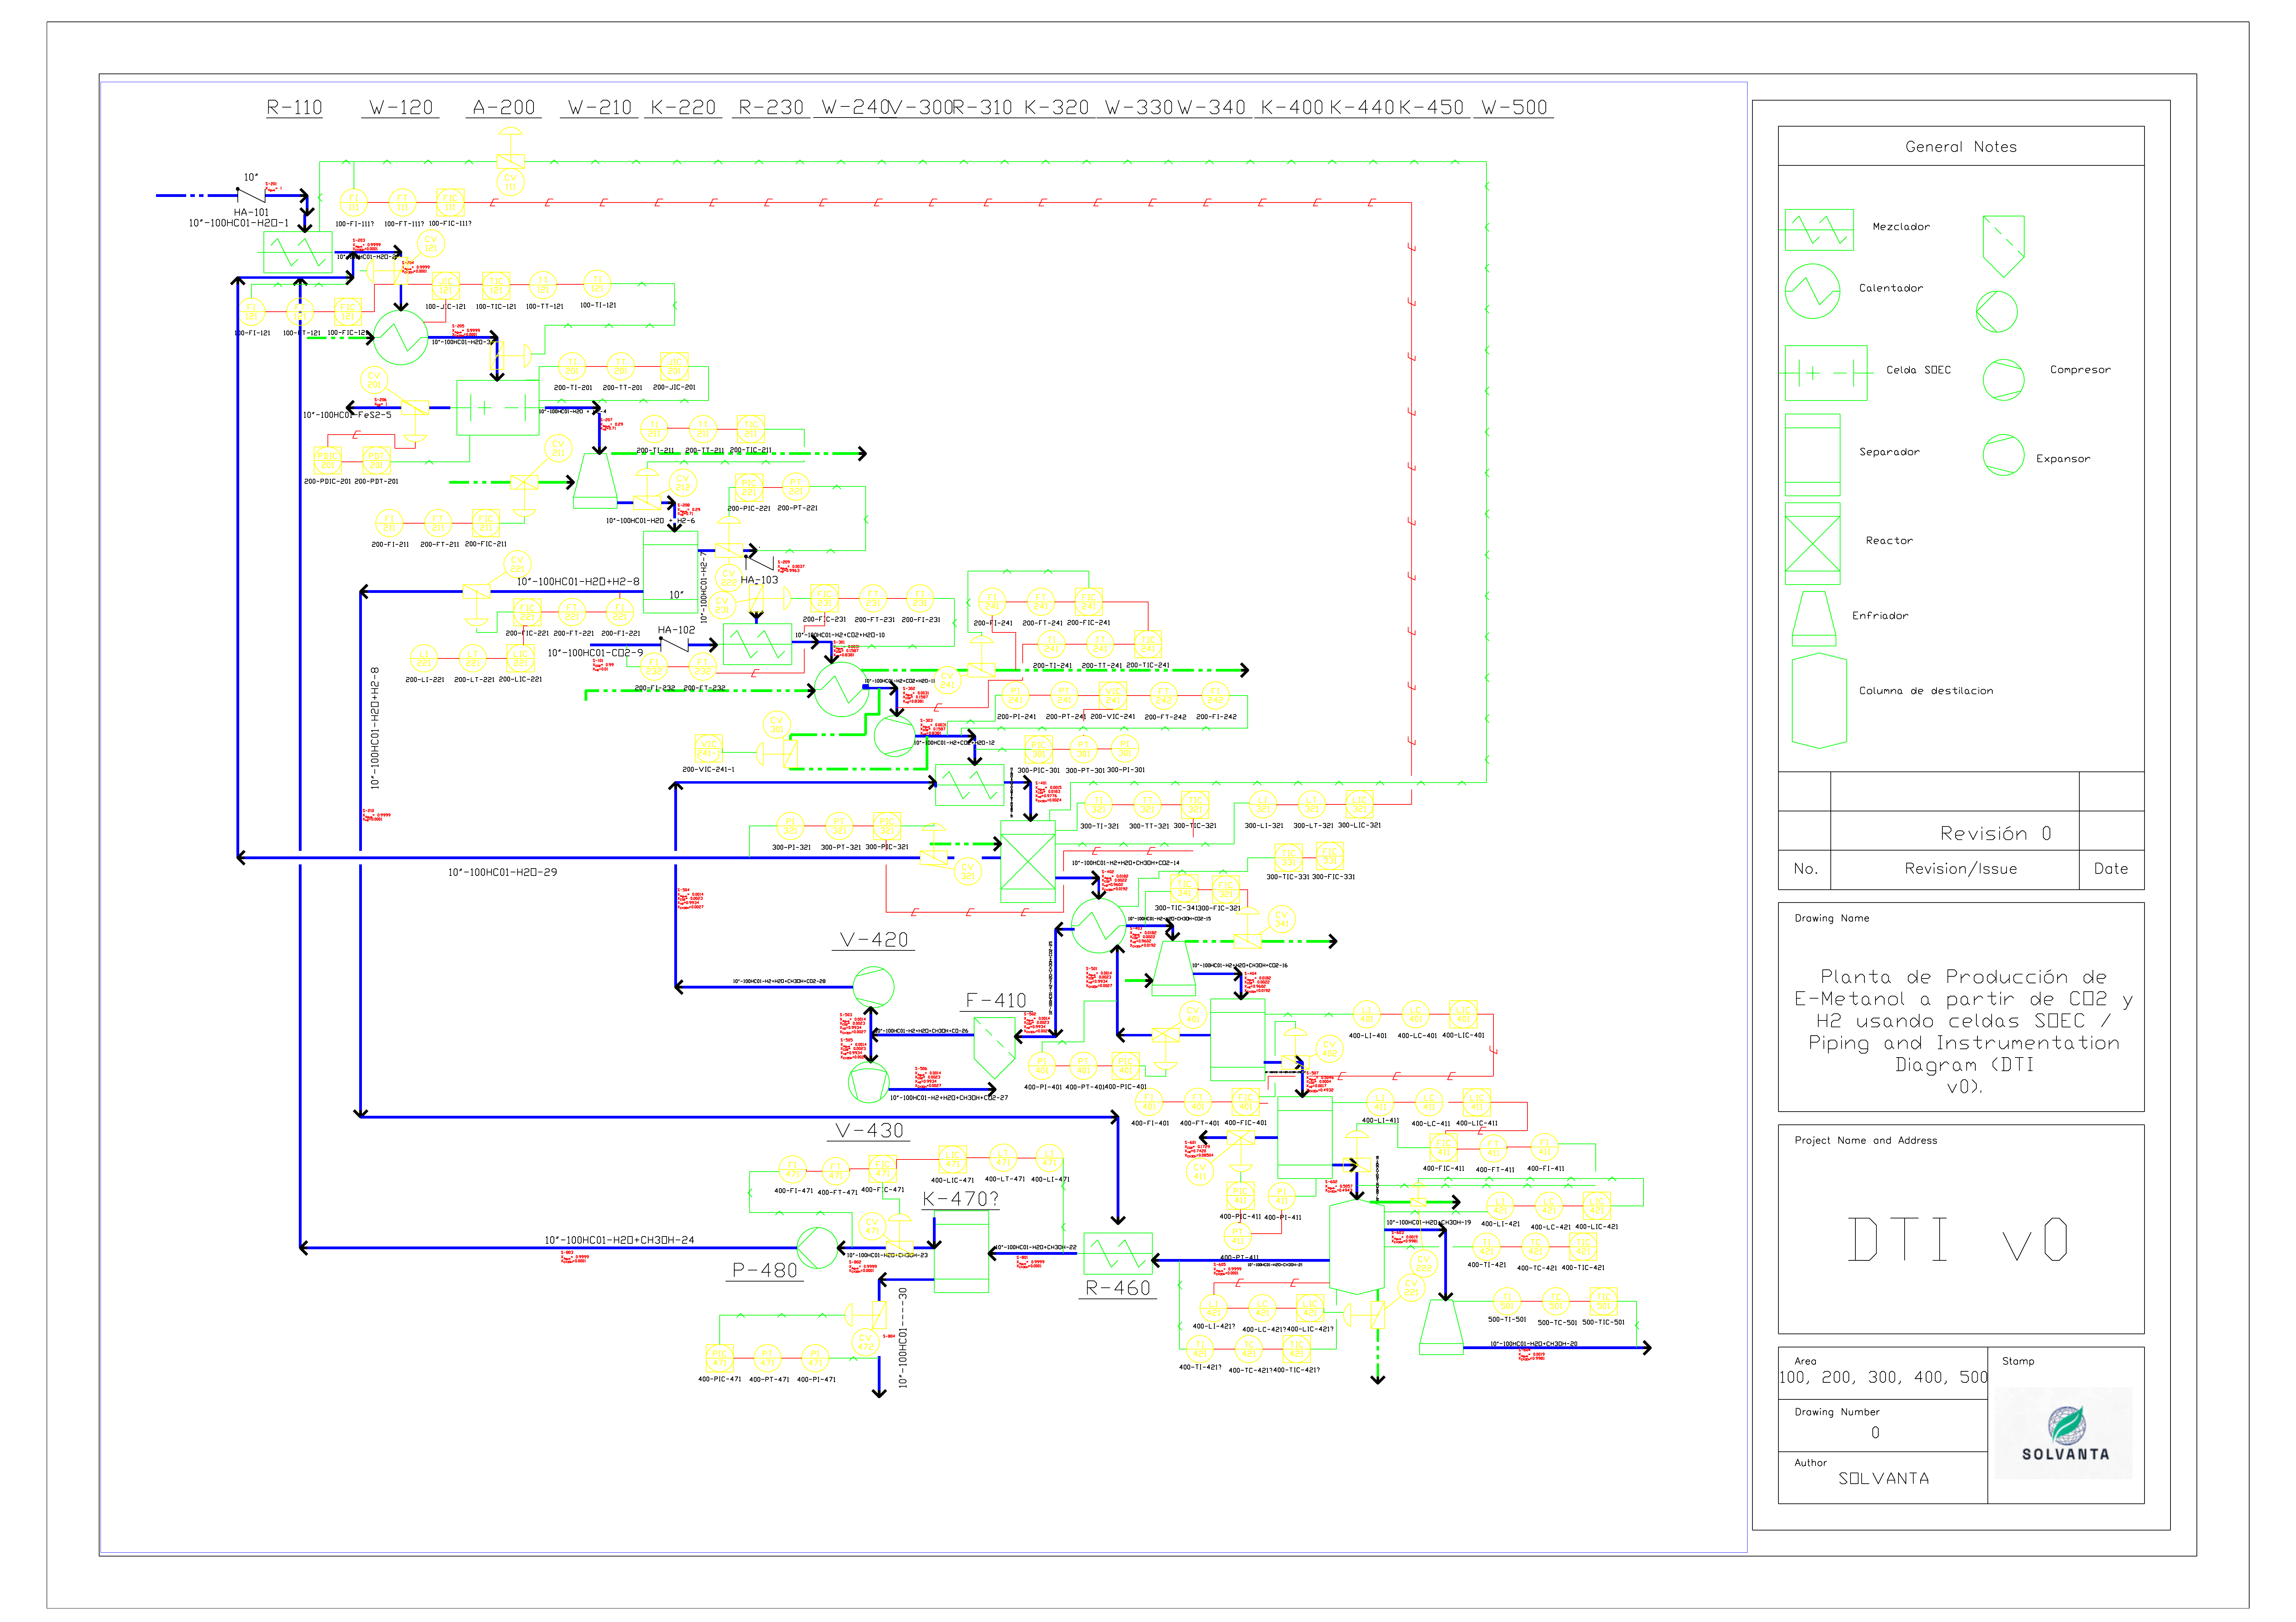
\includegraphics[width=0.95\textwidth]{figuras/dti_v0_preview.png}
    \caption{Diagrama de Tuberías e Instrumentación preliminar de la planta de e-metanol (DTI v0.1 -- Solvanta Engineering Solutions).}
    \label{fig:dti_v0}
\end{figure}

\begin{tcolorbox}[colback=lightbg,colframe=solvantablue,arc=1.5mm,width=0.95\textwidth,boxrule=0.8pt]
    \small \textbf{Consulta del Plano Completo en Alta Resolución:} \\
    El archivo vectorial original del DTI completo en formato PDF puede consultarse directamente en el repositorio GitHub oficial del proyecto, en la ruta real y verificada:
    \begin{center}
        \href{https://github.com/Karoc-cmd/RFP-CCM-EM-001/blob/main/02_Ingenieria_y_Diagramas/DTI_PID/DTI-v0_Solvanta.pdf}{\texttt{02\_Ingenieria\_y\_Diagramas/DTI\_PID/DTI-v0\_Solvanta.pdf}}
    \end{center}
    \footnotesize \textit{Nota de ingeniería:} Las modificaciones derivadas de la presente filosofía FC-01 (lazos compactos, simplificación del expansor X-501, lazos de potencia JIC y conexiones de chaqueta) serán integradas en la próxima emisión del plano (\textbf{DTI v1.0}) posterior a la ejecución de la sesión HAZOP.
\end{tcolorbox}

% ==============================================================================
% SECCIÓN 8: CONCLUSIONES Y REFERENCIAS
% ==============================================================================
\section{Conclusiones}
El desarrollo de la presente Filosofía de Control (\textbf{FC-01}) para la planta de e-metanol ($30\,000\text{ t/año}$) de Solvanta Engineering Solutions permite consolidar las siguientes conclusiones técnicas:
\begin{enumerate}
    \item \textbf{Sólida consistencia fenomenológica y cuantitativa:} Se formularon y estructuraron 28 lazos de control primarios sustentados directamente en los balances de materia y energía y en los parámetros de la simulación rigurosa convergida en DWSIM v1, evitando valores arbitrarios y respetando la evidencia gráfica actual.
    \item \textbf{Integración y simplificación respecto al diseño anterior:} Se implementó con éxito la compactación funcional de instrumentos (FIC, PIC, TIC, LIC, JIC, UIC) y se adoptó la simplificación del lazo del expansor X-501 a un único controlador \texttt{PIC}, eliminando arquitecturas innecesarias del documento histórico EI-01.
    \item \textbf{Preservación de la fidelidad del modelado de equipos:} Se reconoció explícitamente la representación técnica de la chaqueta de R-401 como circuito térmico cerrado integrado con el tambor V-801 y la bomba P-801, así como la naturaleza 100\% eléctrica de los sobrecalentadores E-202 y EL-201 gobernados por controladores de potencia \texttt{JIC}.
    \item \textbf{Priorización rigurosa de seguridad operativa:} Se definieron 5 interlocks candidatos esenciales que resuelven los principales riesgos operacionales: embalamiento térmico en R-401 ($T > 270^\circ\text{C}$), sobrepresión del loop ($P > 82\,\text{bar}$), rotura de membranas en SOEC ($|\Delta P| > 0.5\,\text{bar}$), escape de gas de alta presión en el flash V-501 (*blow-by*) y prevención de surge en compresión.
    \item \textbf{Puente vinculante hacia el DTI v1.0 y HAZOP:} La filosofía FC-01 entrega la especificación completa requerida para actualizar el plano de tuberías e instrumentación hacia la versión DTI v1.0 y constituye el insumo rector indispensable para desarrollar la matriz causa-efecto y el análisis de riesgos HAZOP del proyecto licitado.
\end{enumerate}

\section{Referencias Bibliográficas}
\begin{enumerate}[label={[\arabic*]}]
    \item \textbf{Seborg, D. E., Edgar, T. F., Mellichamp, D. A., \& Doyle, F. J.} (2016). \textit{Process Dynamics and Control} (4th ed.). John Wiley \& Sons, Hoboken, NJ.
    \item \textbf{Smith, C. A., \& Corripio, A. B.} (2006). \textit{Principles and Practice of Automatic Process Control} (3rd ed.). John Wiley \& Sons.
    \item \textbf{Towler, G., \& Sinnott, R.} (2021). \textit{Chemical Engineering Design: Principles, Practice and Economics of Plant and Process Design} (6th ed.). Butterworth-Heinemann.
    \item \textbf{Luyben, W. L.} (2002). \textit{Plantwide Dynamic Simulators in Chemical Processing and Control}. Marcel Dekker, New York.
    \item \textbf{International Society of Automation (ISA).} (2009). \textit{ANSI/ISA-5.1-2009: Instrumentation Symbols and Identification}. ISA, Research Triangle Park, NC.
    \item \textbf{International Electrotechnical Commission (IEC).} (2016). \textit{IEC 61511: Functional safety - Safety instrumented systems for the process industry sector}. IEC, Geneva.
    \item \textbf{American Petroleum Institute (API).} (2020). \textit{API RP 520: Sizing, Selection, and Installation of Pressure-relieving Devices in Refineries}. API Publishing Services, Washington, D.C.
    \item \textbf{DWSIM Chemical Process Simulator.} (2026). \textit{Modelado Termodinámico y Simulación Rigurosa de la Planta de e-Metanol Solvanta (DWSIM v1 Aprobada)}. Solvanta Engineering Solutions S.A. de C.V.
\end{enumerate}

\end{document}
